\subsection{Interaction of particles with matter}
\label{sec:interaction_particle_matter}
In order to detect a particle it must interact with the material of the detector and transfer energy in some recognisable fashion.
\paragraph{Particle detection occurs via the energy loss of particles through the material they traverse.}

\paragraph{Possibilities}
\begin{itemize}
\item[(i)] EM charged particles $\rightarrow$ Ionisation, Bremsstrahlung$^*$, Cherenkov
\item[(ii)] Hadrons $\rightarrow$ Nuclear interactions$^*$ (equivalent to ones above the involving the strong force)
\item[(iii)] Photons $\rightarrow$ Pair production$^{**}$, Photoelectric effect, Compton effect
\end{itemize}
$^{(*)}$ Cause a shower of particles (see later).\newline
$^{(**)}$ Total energy loss via a single interaction converting into charged particles.\newline
Some examples of what these processes look like:

\begin{center}
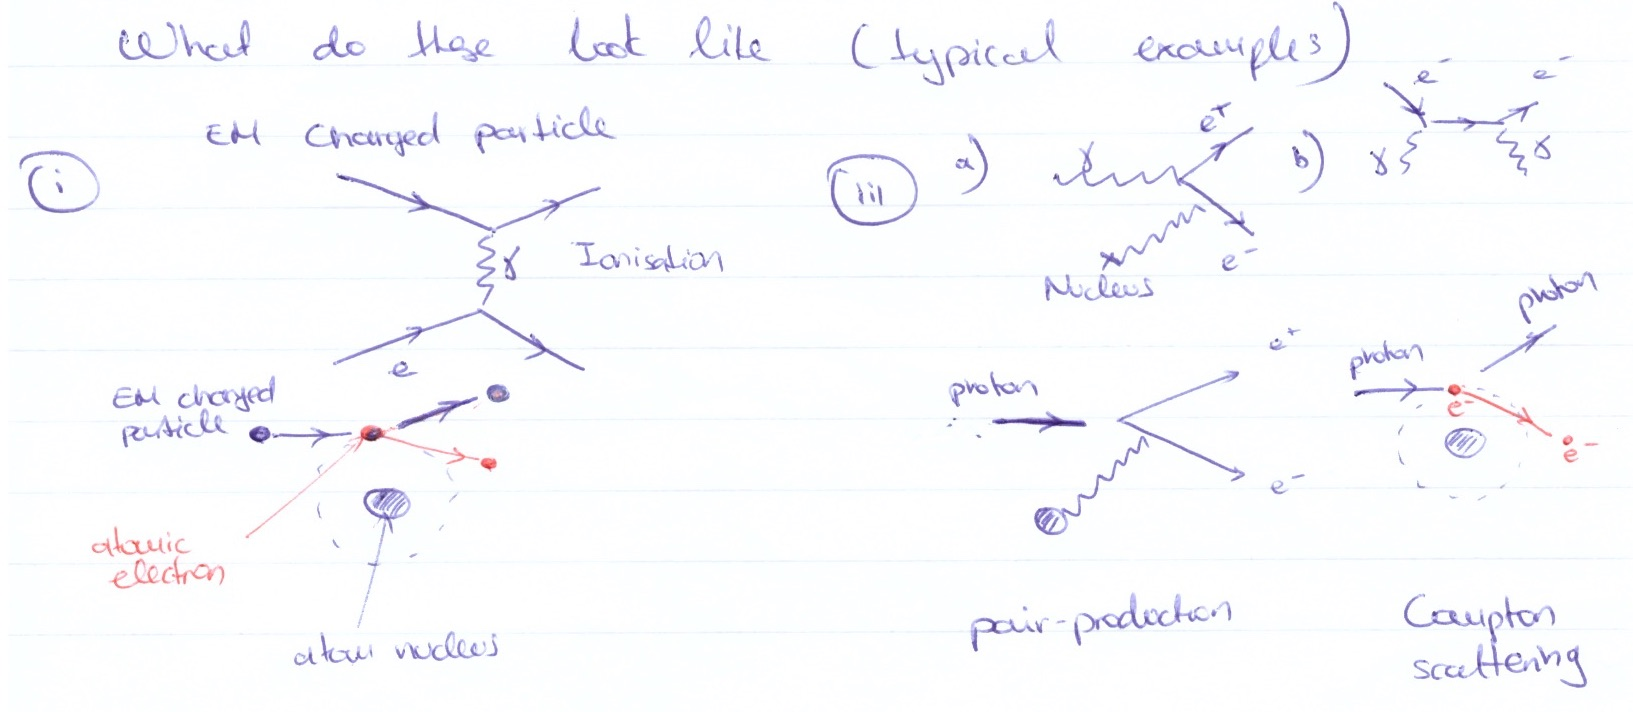
\includegraphics[width=0.95\textwidth]{fig/strongforce/matterinteractions/interactions1.jpg}\newline
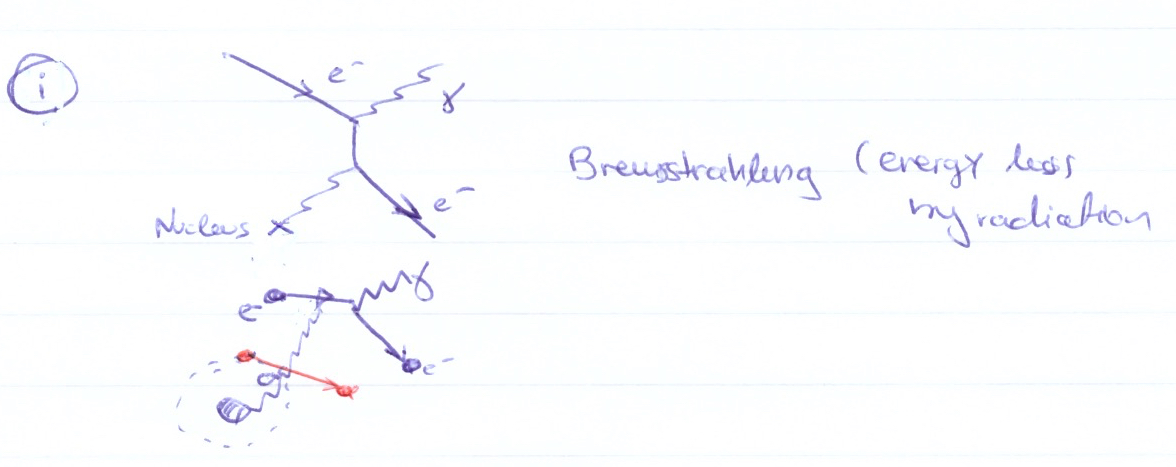
\includegraphics[width=0.8\textwidth]{fig/strongforce/matterinteractions/interactions2.jpg}
\end{center}


\subsubsection{Energy loss by ionisation}
We can quantify the energy loss of a particle traversing through the detector, by looking at the average rate of energy lost per unit distance.


For an incident particle of charge $ze$ with mass $M>>m_e$, losing energy by ionising atomic electrons in a material with atomic number $Z$ we can use the Bethe-Bloch equation:

\begin{equation}
\label{eq:bethebloch}
<\frac{dE}{dx}>\approx -2C\frac{m_ec^2Zz^2}{\beta^2A}\rho\left[\frac{1}{2}\log\frac{2m_ec^2\beta^2\gamma^2T_{\rm max}}{I^2}-\beta^2-\frac{\delta(\beta\gamma)}{2}\right]
\end{equation}
with \[C=2\pi N_A\frac{e^2}{4\pi\epsilon_0m_ec^2}.\] 
$I$ is the mean ionisation potential ie $h<\nu_e>$ (given by $\sim10Z$~eV for $Z>20$), $\rho$ is the density of the material, $\delta(\beta\gamma)$ is a density correction term because the incoming particle can polarise the medium, and $T_{\rm max}$ is the maximum energy transfer in a single collision given by
\[
T_{\rm max}=\frac{2m_ec^2\beta^2\gamma^2}{[1+2\gamma m_e/M +(m_e/M)^2].}
\]
For $\frac{\gamma m_e}{M}<<1$, $T_{\rm max}$ can be simplified to
\[
T_{\rm max}\sim2\gamma^2\beta^2m_ec^2.
\]

\exercise{
One can approximate the picture of a charged particle of mass $M \gg m_e$ with charge $ze$ traversing a material of atomic number $Z$, as an infinitely long cylinder of radius $b$, with charge uniformly distributed  on the surface, surrounding the charged particle which sits in the middle. Let us consider this charged particle interacting with an electron in the medium.
\begin{center}
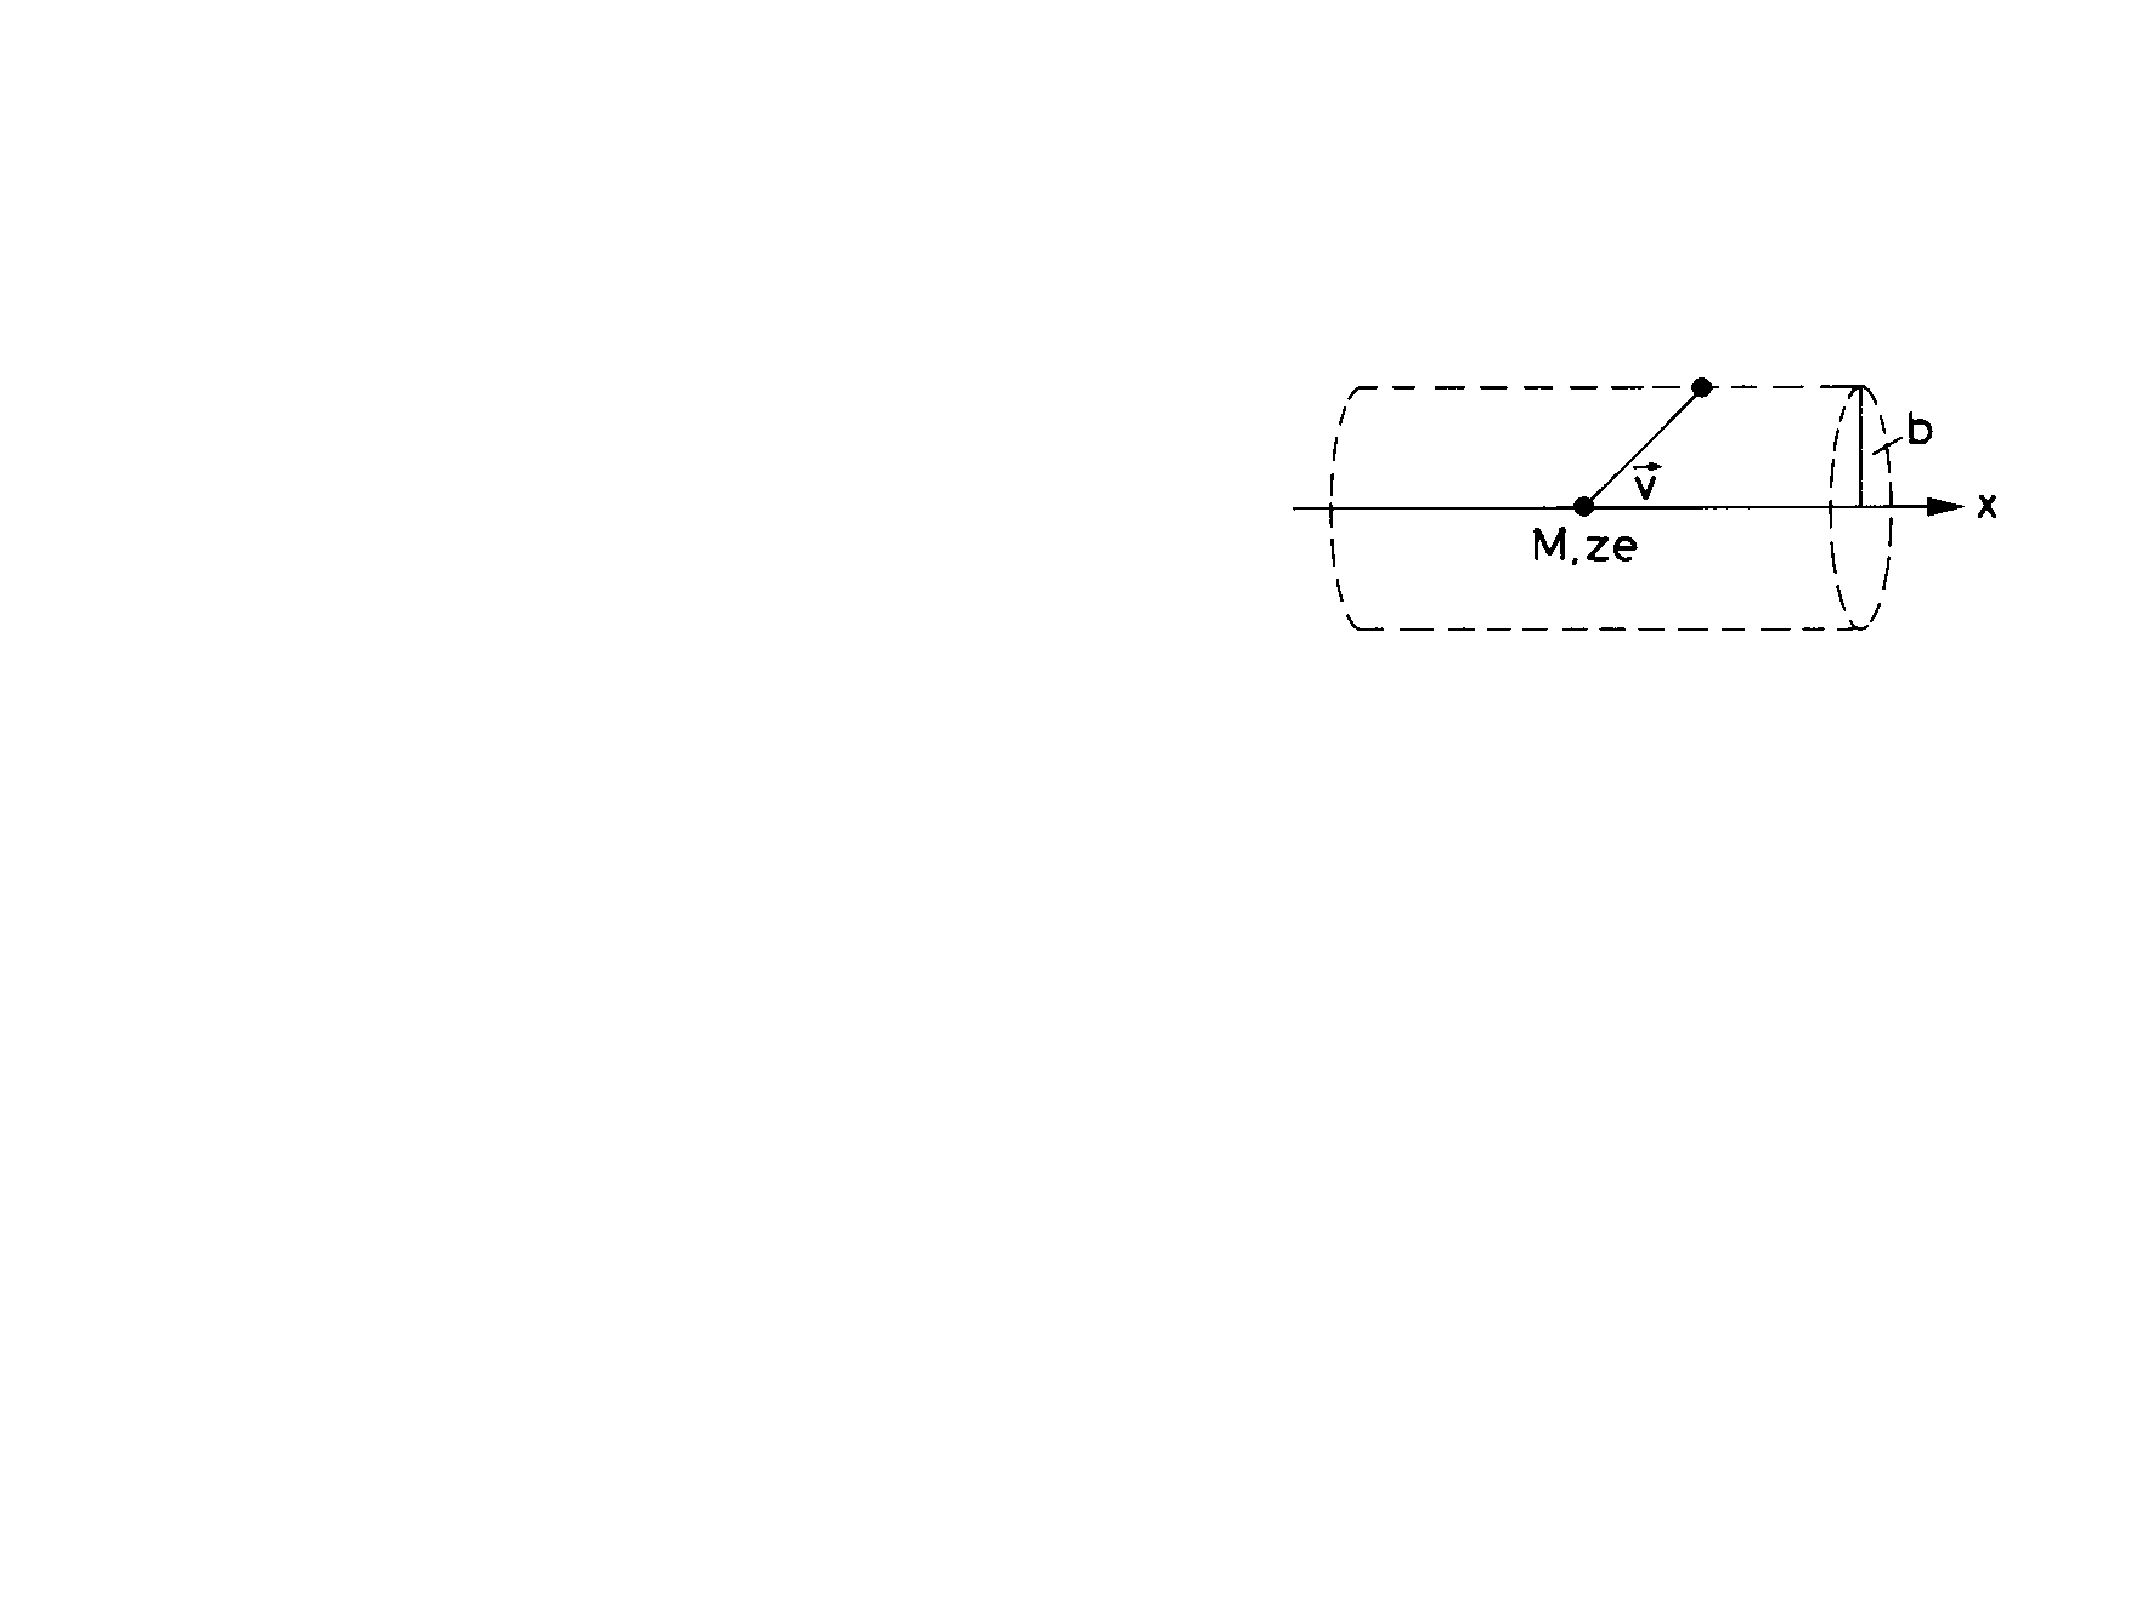
\includegraphics[width=0.5\textwidth]{fig/strongforce/matterinteractions/particle_in_cylinder.pdf}
\end{center}
By applying Gauss's law, show that the momentum transfer perpendicular to the motion of the charged particle, defined by $\Delta p_{\perp}=\int F_{\perp} dt$, is given by $\frac{2ze^2}{bv}$, where $v$ is the speed of the charged particle. Show that $\Delta p_{\parallel}=0$. You can use the fact that in natural units $\epsilon_0=\frac{1}{4\pi}$.\\\\

Consider now a section of this cylinder of length $dx$. Also let's assume the surface of the cylinder has a width $db$. Show that if the electron density of the cylinder in $n$, the number of electrons contained within this cylinder section is $N_e=n(2\pi b)dbdx$. Therefore show that the energy loss per path length $dx$ traversed by the charged particle is given by:
\[dE=-\frac{4\pi n z^2 e^4}{m_e v^2}\frac{db}{b}dx\]
Hint: Energy transferred onto a single electron on surface of cylinder is given by $\Delta E=\frac{\Delta p^2}{2m_e}$\\\\

By integrating between $b_{\rm min}$ and $b_{\rm max}$ we have:
\[
\frac{dE}{dx}=-\frac{4\pi n z^2e^4}{m_ev^2}\log\frac{b_{\rm max}}{b_{\rm min}}
\]
The question now is what are sensible values for $b_{\rm min}$ and $b_{\rm max}$. 
If $b$ becomes so large that the energy transfer is lower than the mean energy required to ionise an electron (given by $I=h<\nu_e>$). The minimum value of $b$ occurs when the maximum possible energy transfer occurs. From relativistic energy-momentum conservation, the maximum energy transferred is $\approx 2\gamma^2\beta^2m_e$ (in natural units)
Therefore show that:
$\displaystyle \frac{dE}{dx}=-\frac{4\pi z^2 e^4}{m_e \beta^2}n\frac{1}{2}\log\frac{2m_e\beta^2\gamma^2}{h<\nu_e>}$
}

\paragraph{Example: Pions in Cu.} Features are common for all materials

\begin{center}
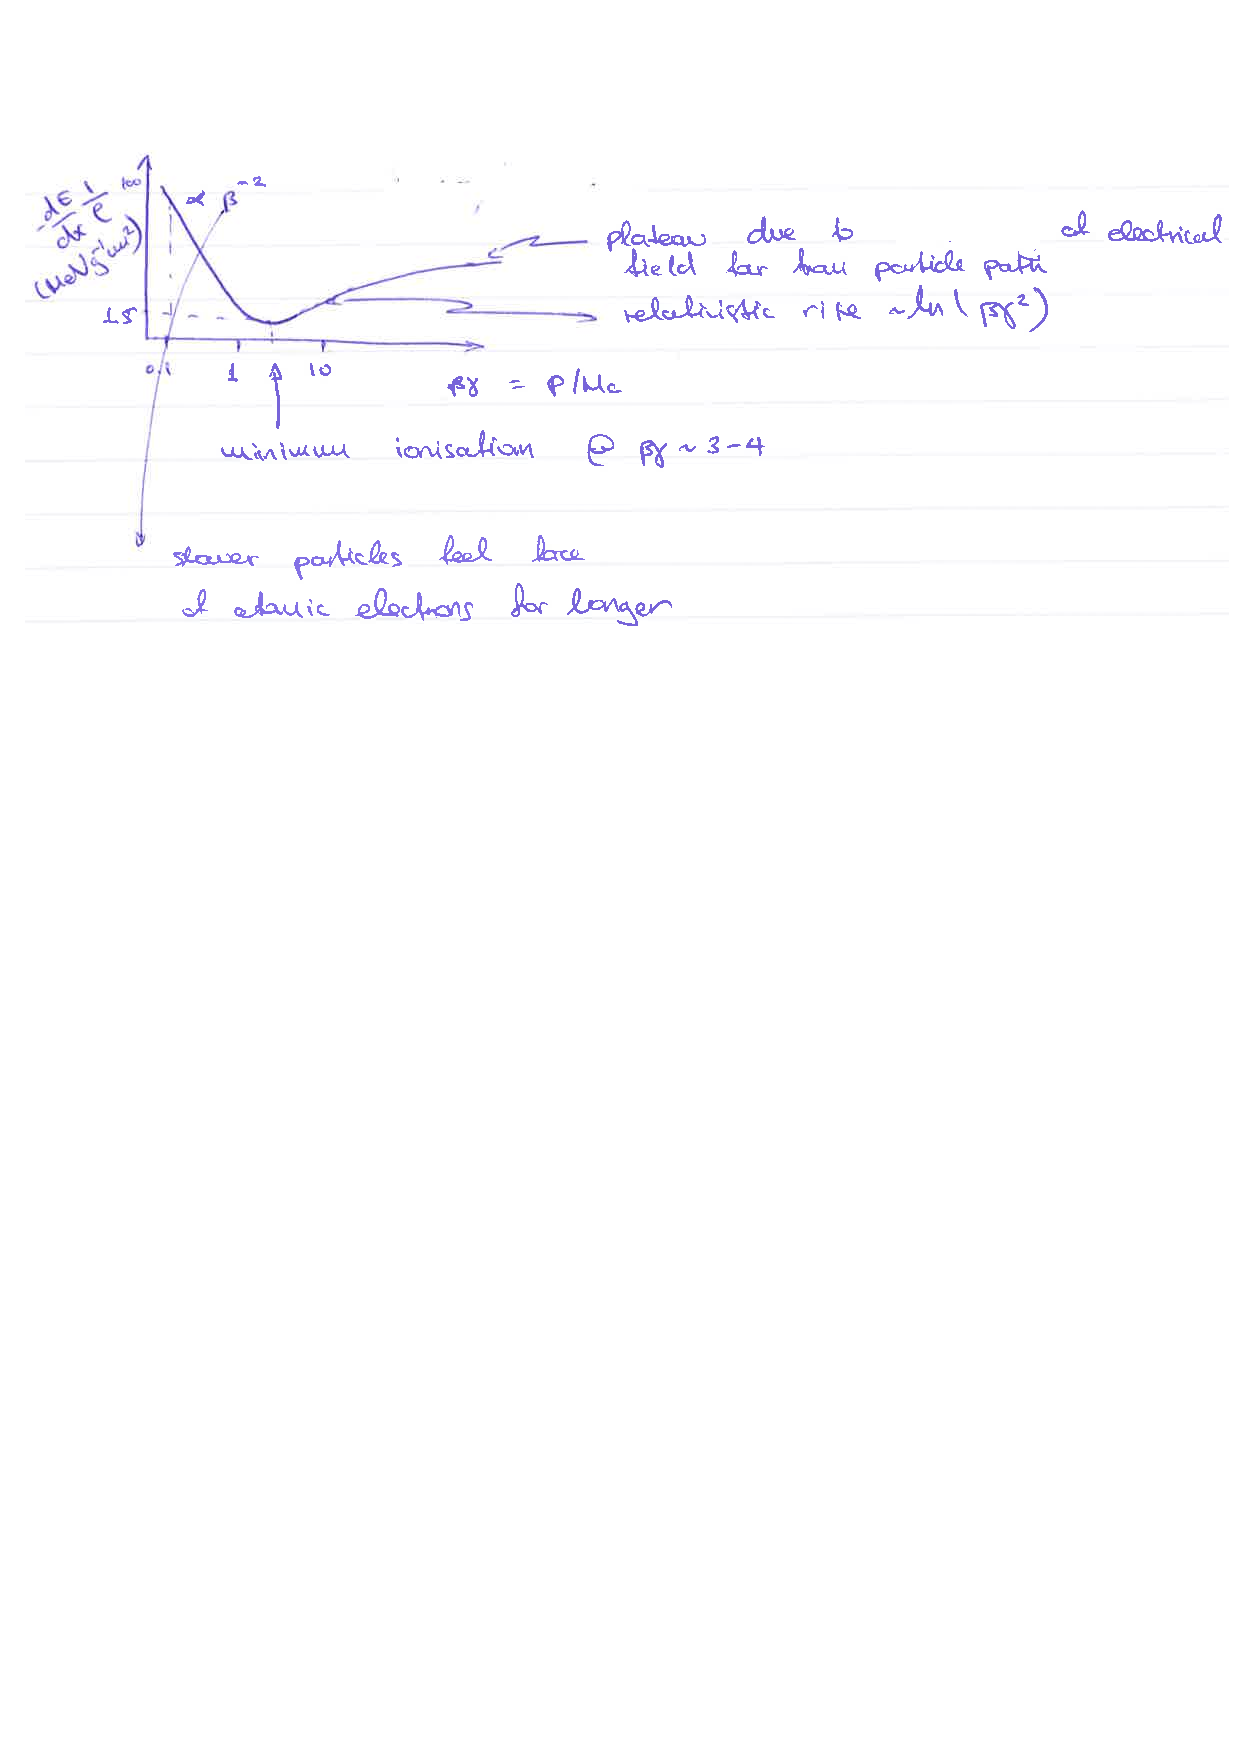
\includegraphics[width=0.95\textwidth]{fig/strongforce/matterinteractions/interactions4.pdf}
\end{center}

Let us consider some key features, ignoring the $-\beta^2$ and $-\delta(\beta\gamma)$ terms for a moment we have:
\[<\frac{dE}{dx}>\propto -\frac{1}{\beta^2}\log{({\rm const}\cdot\beta^2\gamma^2)}.\]
\begin{itemize}
\item The $1/\beta^2$ fall is due to the fact that slower particles feel the force of atomic electrons for longer. 
\item The $\log{({\rm const}}\cdot\beta^2\gamma^2)$ term is a relativistic rise which comes about due to the fact that high energy particles the electric field transverse to the direction of motion of the particle increases, thus increasing the probability of an interaction.
\end{itemize}
The plateau of the $<\frac{dE}{dx}>$ distribution for $\beta\gamma>10$ is due to the fact that the incoming particle polarises the medium thus shielding the electric field far from the particle path, thus cutting the long range contribution. This is the reason behind the $\delta(\beta\gamma)$ term.  

The figure below shows the energy lost via ionisation in a sub-detector of ALICE (A Large Ion Collider Experiment) at CERN. It is evident that if one knows the momentum of the incoming particle, then the energy lost through ionisation can distinguish between different incoming particles.
\begin{center}
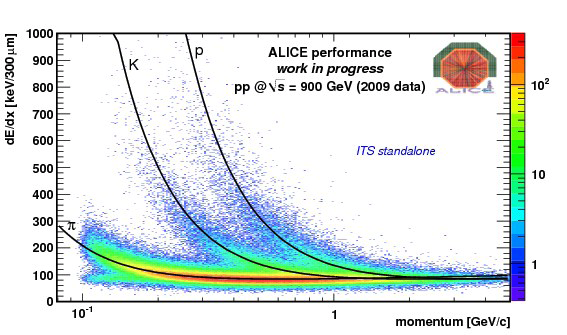
\includegraphics[width=0.95\textwidth]{fig/strongforce/matterinteractions/alice_dedx.png}
\end{center}

\paragraph{Multiple scattering through small angles: time permitting}
A charged particle traversing a medium feels the Coulomb force of nuclei and hence gets deflected. As it gets multiple deflections from multiple nuclei as it traverses the material, this effect is called ``multiple scattering''. The deflection angle follows a Gaussian distribution centred at zero with a width $\theta_0$ given by:
\[
\theta_0\propto \frac{z\sqrt{x}}{vp}(1+0.038\log{x}+{\rm const})
\]
where $z$ is the charge of the particle in multiples of electric charge, $x$ is the distance travelled, $p$ is the momentum and $v$ is the speed of the particle traversing the medium. A pictorial view of the deflection can be seen below.

\begin{center}
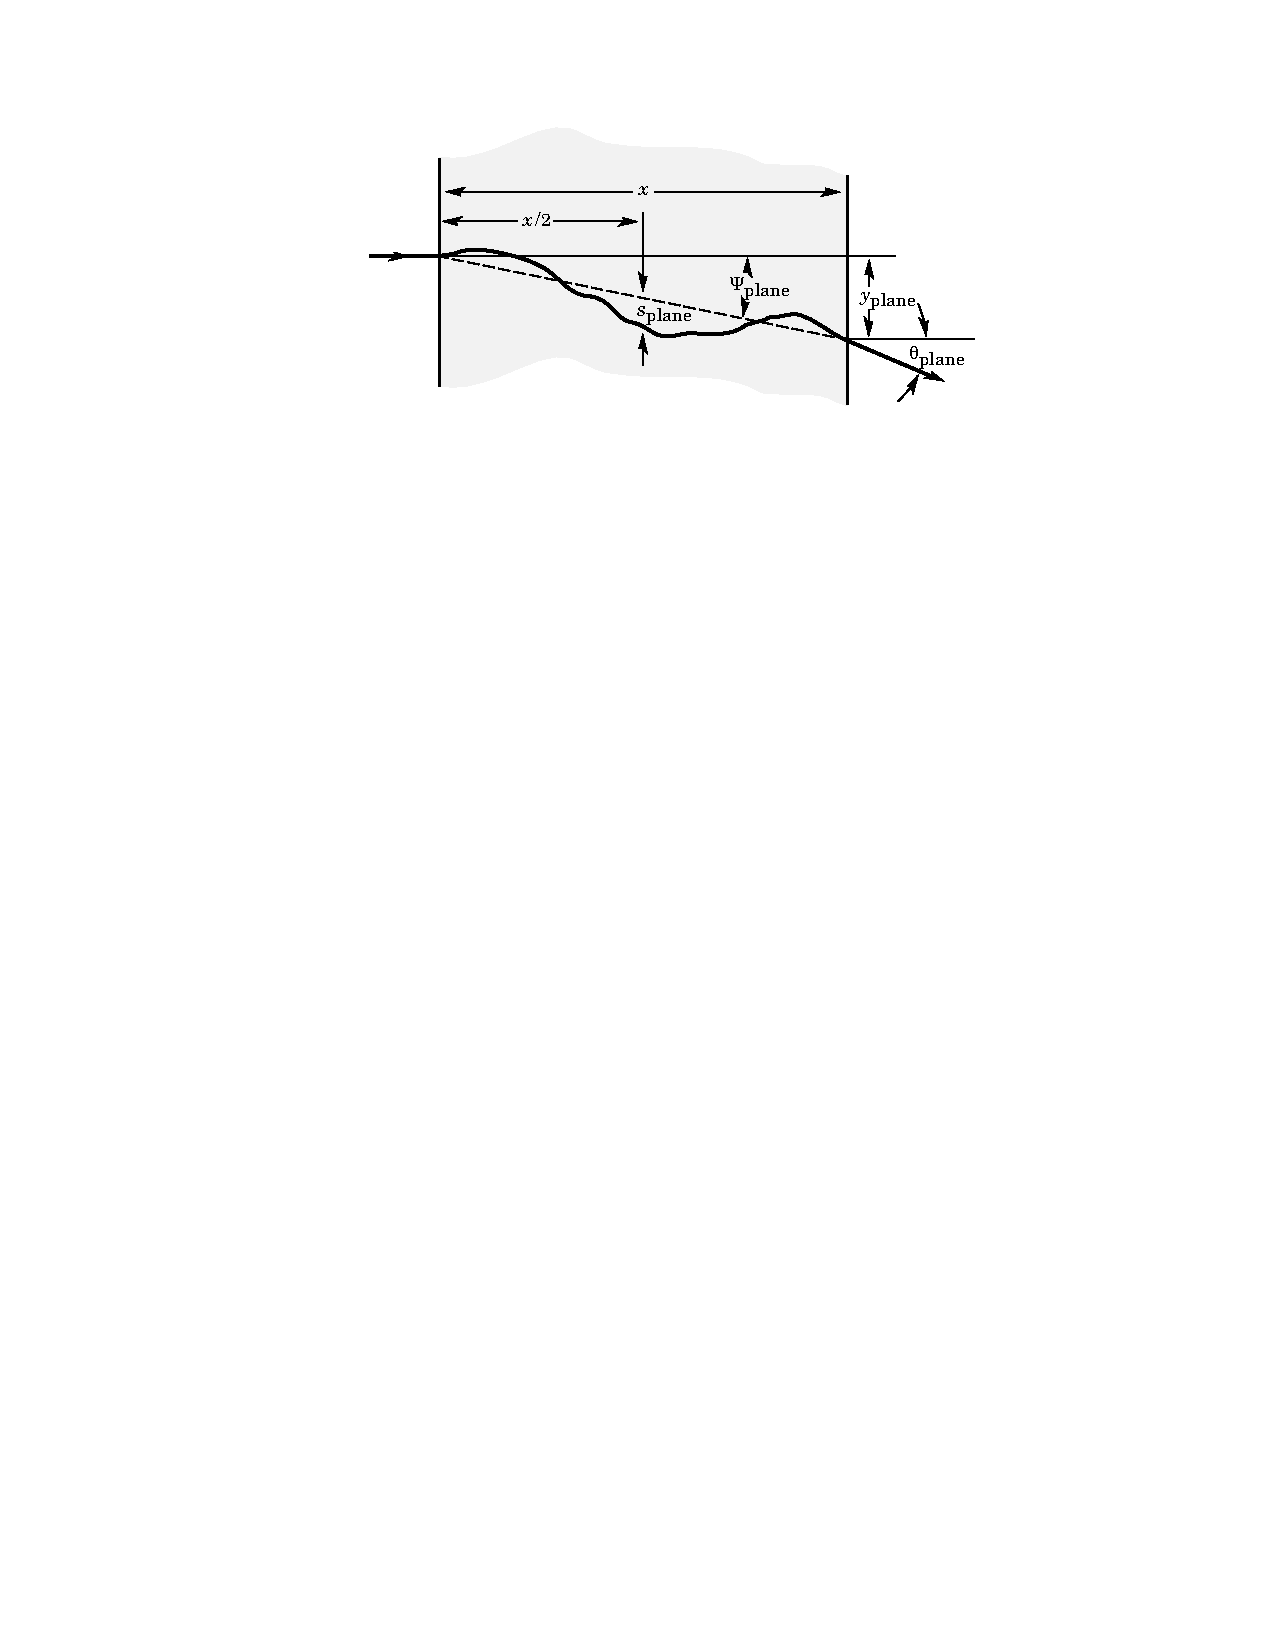
\includegraphics[width=0.95\textwidth]{fig/strongforce/matterinteractions/scattering_angle.pdf}
\end{center}


\paragraph{Particle Range: time permitting}
The range $R$ of a particle is defined as the distance it will travel
in the material before loosing all its energy through ionisation. It is a useful
quantity, however it is not the full picture as particles can loose energy through
other means, as we shall see later in the course.
In any case it is interesting to calculate. 
Suppose a particle enters a material with energy $E_0$. We can therefore define the range as
\[
<R>=\int_{E_0}^{0}\frac{dE}{<dE/dx>}.
\]
Insterting Eq.~\ref{eq:bethebloch}, we get 
\begin{equation}
<R>\propto \frac{E_{0}^{3/2}}{\sqrt{m}}.
\end{equation}
For the case when energy of incoming particle larger than the rest mass we have
\[
<R>\propto (\gamma m v)^{3/2}.
\]

\fbox{\parbox{0.98\textwidth}{
\paragraph{Beyond scope:}
So far we have discussed the average energy loss through ionisation $<\frac{dE}{dx}>$. In fact the actual energy loss scatters around the mean value ie
\begin{center}
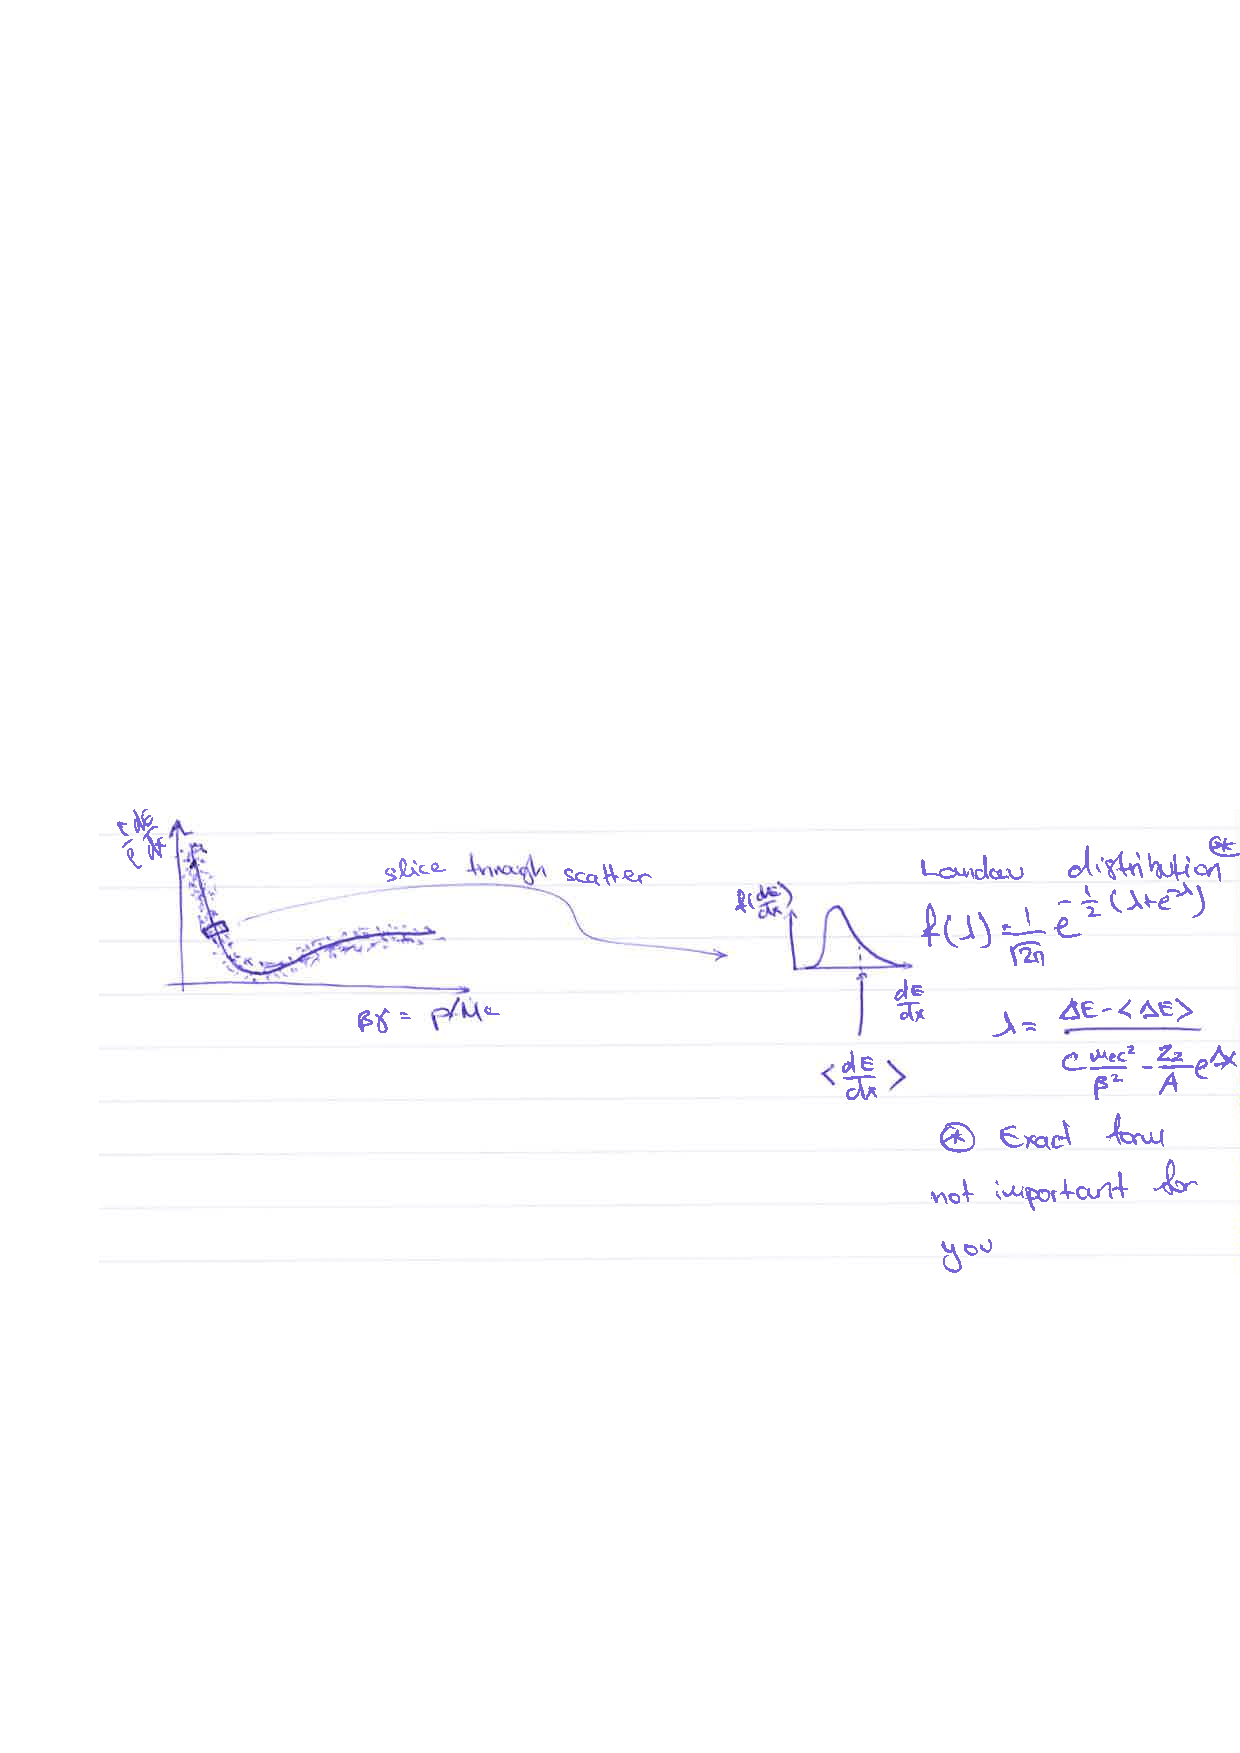
\includegraphics[width=0.95\textwidth]{fig/strongforce/matterinteractions/interactions3.pdf}
\end{center}


}}

